\documentclass[
  11pt,
  letterpaper,
   addpoints,
   answers
  ]{exam}

\usepackage{../exercise-preamble}

\begin{document}

\noindent
\begin{minipage}{0.47\textwidth}

\includegraphics[width=\textwidth]{../fcfm_die}
\end{minipage}
\begin{minipage}{0.53\textwidth}
\begin{center} 
\large\textbf{Electromagnetismo Aplicado} (EL3103-1) \\
\large\textbf{Clase auxiliar 5} \\
\normalsize Prof.~Benjamin Jacard H.\\
\normalsize Prof.~Aux.~Erik Saez A.
\end{center}
\end{minipage}

\vspace{0.5cm}
\noindent
\vspace{.85cm}
\textbf{\underline{Constante de propagación}}: La constante de propagación describe cómo las ondas electromagnéticas se propagan y se atenúan a medida que atraviesan el medio, donde existen dos parámetros de interés 
\begin{itemize}
    \item $\alpha$ : Atenuación del campo electromagnético en el medio. Es la parte real de la constante de propagación.
    \item $j\beta$ :  componente imaginaria de la constante de propagación. Está asociado con la variación espacial de la onda y se mide en radianes por unidad de longitud.
\end{itemize}
La expresión completa viene caracterizada por
\begin{align}
    \gamma = jk = \alpha + j\beta = j\omega \sqrt{\mu \epsilon'\left( 1- j \frac{\epsilon''}{\epsilon'} \right)}
\end{align}
Para la gran mayoría de ejercicios se considerara que los campos eléctricos y magnéticos son perpendiculares a la dirección de propagación y por tanto son representados tal que:
\begin{align}
    \Vec{E}(z,t) = E_{inc}e^{z(\alpha - j\beta)}e^{j\omega t} + E_{ref}e^{z(\alpha +j\beta)}e^{j\omega t}
\end{align}
Donde se tendrá una onda incidente $E_{inc}$ (Que viene de alguna fuente)  y una onda reflejada  $E_{ref}$ (Producto del cambio de medio),  como a su vez una onda que puede ser transmitida que continuara en el otro medio en caso de existir. Ademas debemos considerar que la propagación es en $\hat{k}$ .Sabemos que debido a la notación fasorial podemos expresa el rotor del campo eléctrico como:
\begin{align}
    \nabla \times \Vec{E} = -j\omega\mu_{0}\Vec{H}
\end{align}
Lo que permite obtener el campo $\Vec{H}$ en función de $\Vec{E}$ como : 
\begin{align}
    \Vec{H} = Y\hat{n} \times \Vec{E}
\end{align}
Donde $Y$ representa la admitancia del medio , la cual viene dada por:
\begin{align}
    Y &= Y_{0}\sqrt{\epsilon_{r}}\\
      &= \sqrt{\frac{\epsilon_{medio}}{\mu_{0}}}
\end{align}
Es importante recordar las expresiones asociadas a las condiciones de borde así como de Potencia y energía para los próximos ejercicios. Ademas de las siguientes identidades:
\begin{align}
    sen(z) &= \frac{e^{iz} - e^{-iz}}{2i} & cos(z) = \frac{e^{iz}+ e^{iz}}{2}
\end{align}
\begin{questions}
    %%%%%%%%%%%%%%%%%%%%%%%%%%%%
    \question  Demuestra la ecuacion de Onda y derive una expresión explicita para la velocidad de propagación de una onda electromagnética en el vacio.
    %%%%%%%%%%%%%%%%%%%%%%%%%%%
    \begin{solution}
        Es importante el recordar que los campos eléctricos y magnéticos pueden ser representados mediante ecuaciones de onda. Por ecuaciones de Maxwell se tiene:
\begin{align}
     \Vec{\nabla} \times \Vec{B} &= \epsilon_{0}\mu_{0}\frac{\partial \Vec{E}}{\partial t}\\
\end{align}
Luego esto se utilizara en lo siguiente. Haciendo uso de las propiedades de los operadores.
\begin{align}
    \Vec{\nabla} \times ( \Vec{\nabla} \times \Vec{B}) &= \Vec{\nabla}(\Vec{\nabla} \cdot \Vec{B}) - \nabla^{2}\Vec{B}\\
    \Vec{\nabla} \times ( \Vec{\nabla} \times \Vec{B}) &= - \Vec{\nabla}^{2}\Vec{B}\\
    \Vec{\nabla} \times \left( \epsilon_{0}\mu_{0}\frac{\partial \Vec{E}}{\partial t}\right) &= -\Vec{\nabla}^{2} \Vec{B}\\
    \epsilon_{0} \mu_{0}\left( \Vec{\nabla} \times \frac{\partial \Vec{E}}{\partial t}\right) &= -\Vec{\nabla}^{2}\Vec{B}\\
    \epsilon_{0} \mu_{0} \frac{\partial }{\partial t}\left( \Vec{\nabla} \times \Vec{E} \right) &= -\Vec{\nabla}^{2}\Vec{B}\\
    \epsilon_{0}\mu_{0} \left( -\frac{\partial^{2}B}{\partial t}\right) &= -\nabla^{2}\Vec{B}\\
    \nabla^{2}\Vec{B} - \epsilon_{0}\mu_{0}\frac{\partial^{2}\Vec{B}}{\partial t^{2}}&=0
\end{align}
Con lo que se logra obtener la ecuación de onda que permite describir el campo magnético, es importante notar que $ c= \frac{1}{\sqrt{\epsilon_{0}\mu_{0}}}$ con c la velocidad de la luz . De manera análoga para el campo eléctrico se tendrá:
\begin{align}
    \nabla^{2}\Vec{E}  -\epsilon_{0}\mu_{0}\frac{\partial^{2} \Vec{E}}{\partial t^{2}} = 0
\end{align}
    \end{solution}
    %%%%%%%%%%%%%%%%%%%%%%%%%%%%
    \question  Considere una onda plana cuyo campo eléctrico tiene una magnitud $E_{0}$ y dirección $\hat{i}$ , incidiendo normalmente en una placa dieléctrica perfecta adosada a un plano perfectamente conductor, como se indica la figura .Ademas considere que la frecuencia de operación es $f_{0}$ y el espesor de la placa dieléctrica es d = $\lambda/4$ en que $\lambda$ es la longitud de onda dentro del dieléctrico.
    \begin{enumerate}
        \item Determine los campos totales E(z) y H(z) en todas partes. Ademas bosqueje $\|E(z)\|$ y $\|H(z)\|$ 
        \item Determine el coeficiente de reflexión $\Gamma$(z) en z=-d
        \item  Determine la densidad de potencia (Por unidad de área en el plano xy) incidente y reflejada para cualquier z$<$-d
    \end{enumerate}
    
    \begin{center}
        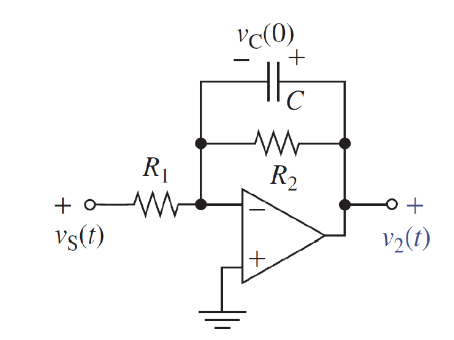
\includegraphics[width=0.5\textwidth]{Auxiliar_5_1}
        \captionof{figure}{Esquema de los dielectricos}
      \end{center}
    %%%%%%%%%%%%%%%%%%%%%%%%%%%%
    \begin{solution}
         \begin{enumerate}
            \item Se busca el obtener los campos E(z) y H(z) en todos los medios , se tendrá que analizar en cada uno de estos, además de analizar sus condiciones de borde:
            \subsubsection*{\underline{Campo eléctrico Medio 1}}
            \begin{align}
                E_{1}(z) = ( E_{1}^{+}e^{jw_{o}t}e^{-jk_{0}z} +E_{1}^{-}e^{jw_{o}t}e^{jk_{0}z})\hat{i}
            \end{align}
            \subsubsection*{\underline{Campo eléctrico Medio 2}}
            \begin{align}
                E_{2}(z) = ( E_{2}^{+}e^{jw_{o}t}e^{-jk_{1}z} +E_{2}^{-}e^{jw_{o}t}e^{jk_{1}z})\hat{i}
            \end{align}
            Luego buscamos analizar las condiciones de borde por tanto se considera los casos en que z = -d y z = 0.
            \subsubsection*{\underline{Caso 1 $E_{1}(z=-d)=E_{2}(z=-d)$}}
            Sabemos por condiciones de borde, que dichos campos eléctricos en la interfaz deberán ser iguales, por lo que igualando se tiene que:
            \begin{align}
                ( E_{1}^{+}e^{jw_{o}t}e^{jk_{0}d} +E_{1}^{-}e^{jw_{o}t}e^{-jk_{0}d})=( E_{2}^{+}e^{jw_{o}t}e^{jk_{1}d} +E_{2}^{-}e^{jw_{o}t}e^{-jk_{1}d})
            \end{align}
            Notamos que la componente asociada a la frecuencia puede ser eliminada , por lo que reduciendo la expresión \textit{(Muchas veces la omitiremos por el mismo motivo dado que entre medios su variante temporal debe ser la misma)} .
            \begin{align}
                ( E_{1}^{+}e^{jk_{0}d} +E_{1}^{-}e^{-jk_{0}d})=( E_{2}^{+}e^{jk_{1}d} +E_{2}^{-}e^{-jk_{1}d})
            \end{align}
            \subsubsection*{\underline{Caso 2 $E_{2}(z=0)=E_{3}(z=0)$ }}
            Se tendrá una condición de conductividad infinita, eso implicara que no existirá onda transmitida y por lo tanto se tendrá directamente que $E_{3} = 0$, es decir:
            \begin{align}
                ( E_{2}^{+}e^{jw_{o}t}e^{-jk_{1}\cdot 0} +E_{2}^{-}e^{jw_{o}t}e^{jk_{1}\cdot 0})= E_{3} &= 0 \\
                E_{2}^{+} + E_{2}^{-} &= 0 \\
                E_{2}^{+} &=  -  E_{2}^{-}
            \end{align}
            Lo cual es consistente con el hecho de que no se esta transmitiendo campo eléctrico en el medio 3 , por lo que las amplitudes incidente y reflejada deben ser iguales y por tanto no existe perdida. Luego deberemos obtener mas ecuaciones para poder encontrar las expresiones particulares de los campos eléctricos , esto se logra relacionando las ecuaciones de intensidad magnética , y teniendo en consideración que son perpendiculares:
            \subsubsection*{\underline{Intensidad de campo magnético para ambos medios }}
            \begin{align}
                H_{1} = Y_{0}(\hat{k}) \times ( E_{1}^{+}e^{jw_{o}t}e^{-jk_{0}z}) (\hat{i}) + Y_{0}(-\hat{k}) \times ( E_{1}^{-}e^{jw_{o}t}e^{jk_{0}z})(\hat{i}) 
            \end{align}
            Dado que sabemos que la propagación va en $\hat{z}$, luego se tendrá que H deberá ir en $\hat{j}$, lo cual es consistente con la expresión anterior:
            \begin{align}
                H_{1}= ( Y_{0}E_{1}^{+}e^{jw_{o}t}e^{-jk_{0}z} - Y_{0} E_{1}^{-}e^{jw_{o}t}e^{jk_{0}z})(\hat{j})
            \end{align}
            Análogamente se tiene que para el medio 2 
            \begin{align}
                H_{2}= ( Y_{1}E_{2}^{+}e^{jw_{o}t}e^{-jk_{1}z} - Y_{1} E_{2}^{-}e^{jw_{o}t}e^{jk_{1}z})(\hat{j})
            \end{align}
            Bajo el mismo argumento anterior tendremos que las intensidades de campo magnético deberán ser iguales y por lo tanto:
            \subsubsection*{\underline{Caso 2 $H_{1}(z=-d)=H_{2}(z=-d)$ }}
            Utilizando la igualdad se obtiene que:
            
            \begin{align}
                  ( Y_{0}E_{1}^{+}e^{jk_{0}d} - Y_{0} E_{1}^{-}e^{-jk_{0}d}) &= ( Y_{1}E_{2}^{+}e^{jk_{1}d} - Y_{1} E_{2}^{-}e^{-jk_{1}d})
            \end{align}
            \begin{align}
                   Y_{0}(E_{1}^{+}e^{jk_{0}d}-E_{1}^{-}e^{-jk_{0}d}) - Y_{1}(E_{2}^{+}e^{jk_{1}d} - E_{2}^{-}e^{-jk_{1}d})&=0
            \end{align}
            Dada la expresión general, nos enfocaremos en el caso particular  d= $\lambda/4$ , por lo que reemplazando sobre las ecuaciones anteriores y recordando que:
            \begin{align}
                k_{0}=\beta = \frac{2\pi}{\lambda}
            \end{align}
            Luego
            \begin{align}
                d\cdot k_{0} = \frac{\lambda}{4} \cdot  \frac{2\pi}{\lambda}
                 = \frac{\pi}{2}
            \end{align}
            Por lo que tenemos que:
            \begin{align}
                e^{\pm j\frac{\pi}{2}} =  \pm j
            \end{align}
            Por lo que reemplazando sobre lo anterior:
            \begin{align}
                E_{1}^{+}j - E_{1}^{-}j =& E_{2}^{+}j - E_{2}^{-}j\\
                 E_{1}^{+} - E_{1}^{-} =& E_{2}^{+} - E_{2}^{-}
            \end{align}
            Pero anteriormente se verifico que $E_{2}^{-} = -E_{2}^{+} $ , por lo que reemplazando tenemos:
            \begin{align}
                E_{1}^{+} - E_{1}^{-} = 2E_{2}^{+}
            \end{align}
            Por otro lado tenemos que para la intensidad de campo magnético sigue que:
            \begin{align}
                 Y_{0}(E_{1}^{+}e^{jk_{0}d}-E_{1}^{-}e^{-jk_{0}d}) &= Y_{1}(E_{2}^{+}e^{jk_{1}d} - E_{2}^{-}e^{-jk_{1}d})\\
                Y_{0}(E_{1}^{+}j+E_{1}^{-}j) &= Y_{1}(E_{2}^{+}j +E_{2}^{-}j)\\
                Y_{0}(E_{1}^{+}+E_{1}^{-}) &= Y_{1}(E_{2}^{+} +E_{2}^{-})\\
                Y_{0}(E_{1}^{+}+E_{1}^{-})&= Y_{1}(E_{2}^{+} +E_{2}^{-})=0\\
                E_{1}^{+} &= -E_{1}^{-}
            \end{align}
            Tenemos además que $E_{1}^{+}=E_{0}$ por lo tanto:
            \begin{align}
                E_{0}= -E_{1}^{-} 
            \end{align}
            De esta forma,
            \begin{align}
                E_{1}^{+} - E_{1}^{-} &= 2E_{2}^{+}\\
                E_{0} + E_{0} &= 2E_{2}^{+}\\
                E_{0} &= E_{2}^{+}
            \end{align}
            Finalmente los campos serán de la siguiente forma (\textit{Utilizaremos las expresiones de seno y coseno vistas en el resumen)}:
            \begin{align}
                E_{1}(z) &= E_{0}e^{-jk_{0}z} + E_{1}^{-}e^{jk_{0}z}\\
                  &=E_{0}e^{-jk_{0}z} - E_{0}^{-}e^{jk_{0}z}\\
                  &= E_{0}(E_{0}e^{-jk_{0}z} - E_{0}^{-}e^{jk_{0}z})\\
                  &= -2jE_{0} sen(k_{0}z)
            \end{align}
            \begin{align}
                E_{2}(z) &= E_{2}^{+}e^{-jk_{1}z} + E_{2}^{-}e^{jk_{1}z}\\
                  &=E_{2}^{+}e^{-jk_{1}z} - E_{2}^{+}e^{jk_{1}z}\\
                  &= E_{2}^{+}(e^{-jk_{1}z} - e^{jk_{1}z})\\
                  &= -2jE_{0} sen(k_{1}z)
            \end{align}
            Por otro lado para la intensidad de campo magnético tenemos que :
            \begin{align}
                H_{1}(z) &= Y_{0}E_{1}^{+}e^{-jk_{0}z} - Y_{0}E_{1}^{-}e^{jk_{0}z}\\
                &= Y_{0}E_{0}^{+}e^{-jk_{0}z} + Y_{0}E_{0}^{-}e^{jk_{0}z}\\
                &= Y_{0}E_{0}(e^{-jk_{0}z} + e^{jk_{0}z} )\\
                &=2Y_{0}E_{0}cos(k_{0}z)
            \end{align}
            \begin{align}
                H_{2}(z) &= Y_{1}E_{2}^{+}e^{-jk_{1}z} - Y_{1}E_{2}^{-}e^{jk_{1}z}\\
                &= Y_{1}E_{2}^{+}e^{-jk_{0}z} + Y_{1}E_{2}^{-}e^{jk_{0}z}\\
                &= Y_{1}E_{0}(e^{-jk_{0}z} + e^{jk_{0}z} )\\
                &=2Y_{1}E_{0}cos(k_{1}z)
            \end{align}
            Con lo que se obtienen finalmente los campos E(z,t) y H(z,t) para ambos medios, luego graficando tenemos lo siguiente:
            \begin{center}
                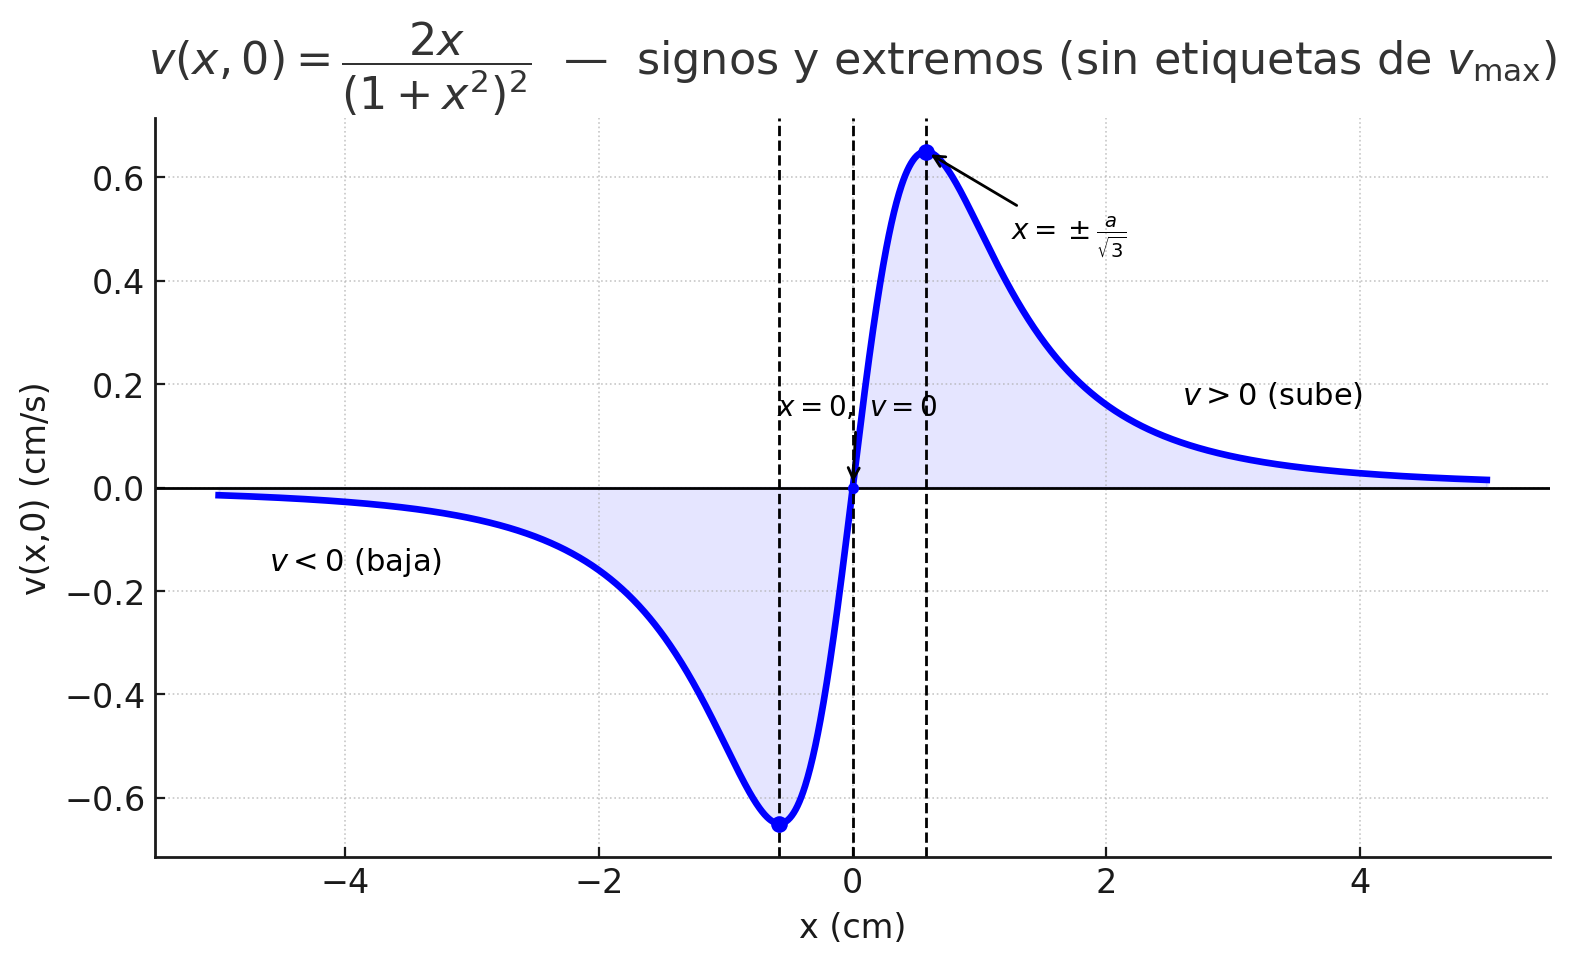
\includegraphics[width=0.6\textwidth]{Auxiliar_5_2}
                \label{fig:mesh25}
            \end{center}.
            \item Se busca determinar el coeficiente de reflexión en $\Gamma$ ,lo obtendremos de manera general (\textit{Es posible obtenerlo directamente de lo visto anteriormente, pero por completitud se obtendrá la expresión general }), por lo que volviendo sobre las ecuaciones anteriores:
            \begin{align}
                ( E_{1}^{+}e^{jk_{0}d} +E_{1}^{-}e^{-jk_{0}d})=( E_{2}^{+}e^{jk_{1}d} +E_{2}^{-}e^{-jk_{1}d})
            \end{align}
            De las relaciones anteriores se obtiene $(E_{2}^{-} = E_{2}^{+}$),
            \begin{align}
                ( E_{1}^{+}e^{jk_{0}d} +E_{1}^{-}e^{-jk_{0}d})&=( E_{2}^{+}e^{jk_{1}d} +E_{2}^{-}e^{-jk_{1}d}) \\&= 2jE_{2}^{+}sen(k_{1}d)\\
                ( E_{1}^{+}e^{jk_{0}d} +E_{1}^{-}e^{-jk_{0}d})&= 2jE_{2}^{+}sen(k_{1}d)
            \end{align}
            En relación a la intensidad de campo magnético.
            \begin{align}
                Y_{0}E_{0}e^{jk_{0}d} - Y_{0}E_{1}^{-}e^{-jk_{o}d}= 2Y_{1}E_{2}^{+}cos(k_{1}d)
            \end{align}
            Recordemos que el coeficiente de reflexión vendrá dado por 
            \begin{align}
                \Gamma(z) &= \frac{E_{1}^{-}e^{-jk_{o}z}}{E_{1}^{+}e^{jk_{o}z}}\\
                          &= \frac{E_{1}^{-}}{E_{1}^{+}} e^{-j2k_{0}d}
            \end{align}
            Es por esto que nos interesa dejar esta relación en términos de expresiones conocidas, en particular de  $E_{1}^{-}$ con respecto a $E_{0}= E_{1}^{+}$ , por lo que debemos despejar el termino reflejado ($E_{1}^{-}$) dividiendo las ecuaciones anteriores, se obtiene lo siguiente:
            \begin{align}
                \frac{E_{1}^{+}e^{jk_{0}d} +E_{1}^{-}e^{-jk_{0}d}}{ Y_{0}(E_{0}e^{jk_{0}d} - E_{1}^{-}e^{-jk_{o}d})}= \frac{1}{Y_{1}}jtan(k_{1}d)
            \end{align}
            Luego despejando $E_{1}^{-}$ tendremos la siguiente expresión:
            \begin{align}
                E_{1}^{-} = E_{0}e^{j2k_{0}d}\frac{\left(\frac{Y_{0}}{Y_{1}} jtg(k_{1}d) -1\right)}{\left(\frac{Y_{0}}{Y_{1}}jtg(k_{1}d) + 1\right)}
            \end{align}
            Que reemplazando sobre la ecuación del coeficiente de reflexión:
            \begin{align}
                \Gamma(z=-d) =  \frac{\left(\frac{Y_{0}}{Y_{1}} jtg(k_{1}d) -1\right)}{\left(\frac{Y_{0}}{Y_{1}}jtg(k_{1}d) + 1\right)}
            \end{align}
            Donde utilizando la siguiente relación:
            \begin{align}
                Y_{0}&= \frac{1}{Z_{0}} & Y_{1}= \frac{1}{Z_{1}}
            \end{align}
            Tal que la expresión:
            \begin{align}
                \Gamma(z = -d) = \frac{jZ_{1}tg(k_{1}d)-Z_{0}}{jZ_{1}tg(k_{1}d) + Z_{0}} 
            \end{align}
            Se obtiene una expresión muy útil que se utilizara mas adelante \textit{(En la siguiente unidad)}, y nos da una expresión que permite obtener el coeficiente de reflexión en cualquier punto que sea de interés, por ahora nos reduciremos a evaluarla en  $d=\lambda/4$ por lo que se obtiene:
            \begin{align}
                 \Gamma(z = -\frac{\lambda}{4}) &= \frac{jZ_{1}tg(k_{1}\frac{\lambda}{4})-Z_{0}}{jZ_{1}tg(k_{1}\frac{\lambda}{4}) + Z_{0}} \\
                 &= 1 
            \end{align}
            Luego,  tendremos que cuando $d=\frac{\lambda}{4}$ ,  el modulo de las amplitudes del campo reflejado y transmitido son iguales y en la misma fase con respecto a la onda incidente.
            \item Se busca obtener la densidad de potencia (Por unidad de área en plano \textit{xy}) por tanto se utilizara el vector de Poynting tal que:
            \begin{align}
                P_{1}^{+}&= \frac{1}{2}Re(E_{1} \times H_{1}^{*} )\hat{k}\\
                         &=\frac{1}{2}Re( E_{0}e^{-jk_{0}z} \times Y_{1}E_{0}e^{jk_{0}z})\\
                         &= \frac{1}{2}Re(E_{0}^{2}Y_{0})\\
                         &= \frac{1}{2}E_{0}^{2}Y_{0}
            \end{align}
            De manera similar tenemos que para la potencia reflejada:
            \begin{align}
                P_{1}^{-} = \frac{1}{2}Re(E_{1}^{-} \times H_{1}^{-}*) (-\hat{k})= \frac{1}{2}Y_{0}E_{0}^{2}
            \end{align}
         \end{enumerate}
    \end{solution}
    %%%%%%%%%%%%%%%%%%%%%%%%%%%
    \question  Considere una onda plana cuyo campo eléctrico tiene una magnitud \(E_0\) y dirección \(\Vec{x}\), incidiendo normalmente en una sección de tres medios diferentes, siendo este último una placa dieléctrica perfecta adosada a un plano perfectamente conductor (\(\sigma = \infty\)), como se indica en el esquema.
    \begin{enumerate}
        \item Obtenga una relación entre los campos \(E^{-}_{2}\) y \(E^{+}_{2}\) en función de \(d_2\).
        \item Una vez determinada la expresión anterior, analice cuando \(d_{2} = \frac{\lambda}{2}\) y explique en términos del módulo del coeficiente de reflexión.
        \item Considerando que \(d_{2} = \frac{\lambda}{2}\), determine una expresión para las amplitudes de los campos \(E^{-}_{1}\) y \(E^{+}_{1}\) y analice el caso cuando \(d_{1} = \frac{\lambda}{2}\).
        \item Considerando que \(d_{1} = d_{2} = \frac{\lambda}{2}\), calcule el valor de potencia por unidad de área en el Medio 1 tanto para la onda incidente como para la reflejada.
        \item ¿Son las potencias para la onda incidente y reflejada, obtenidas con anterioridad, diferentes? Argumente su respuesta.
    \end{enumerate}
    \begin{center}
        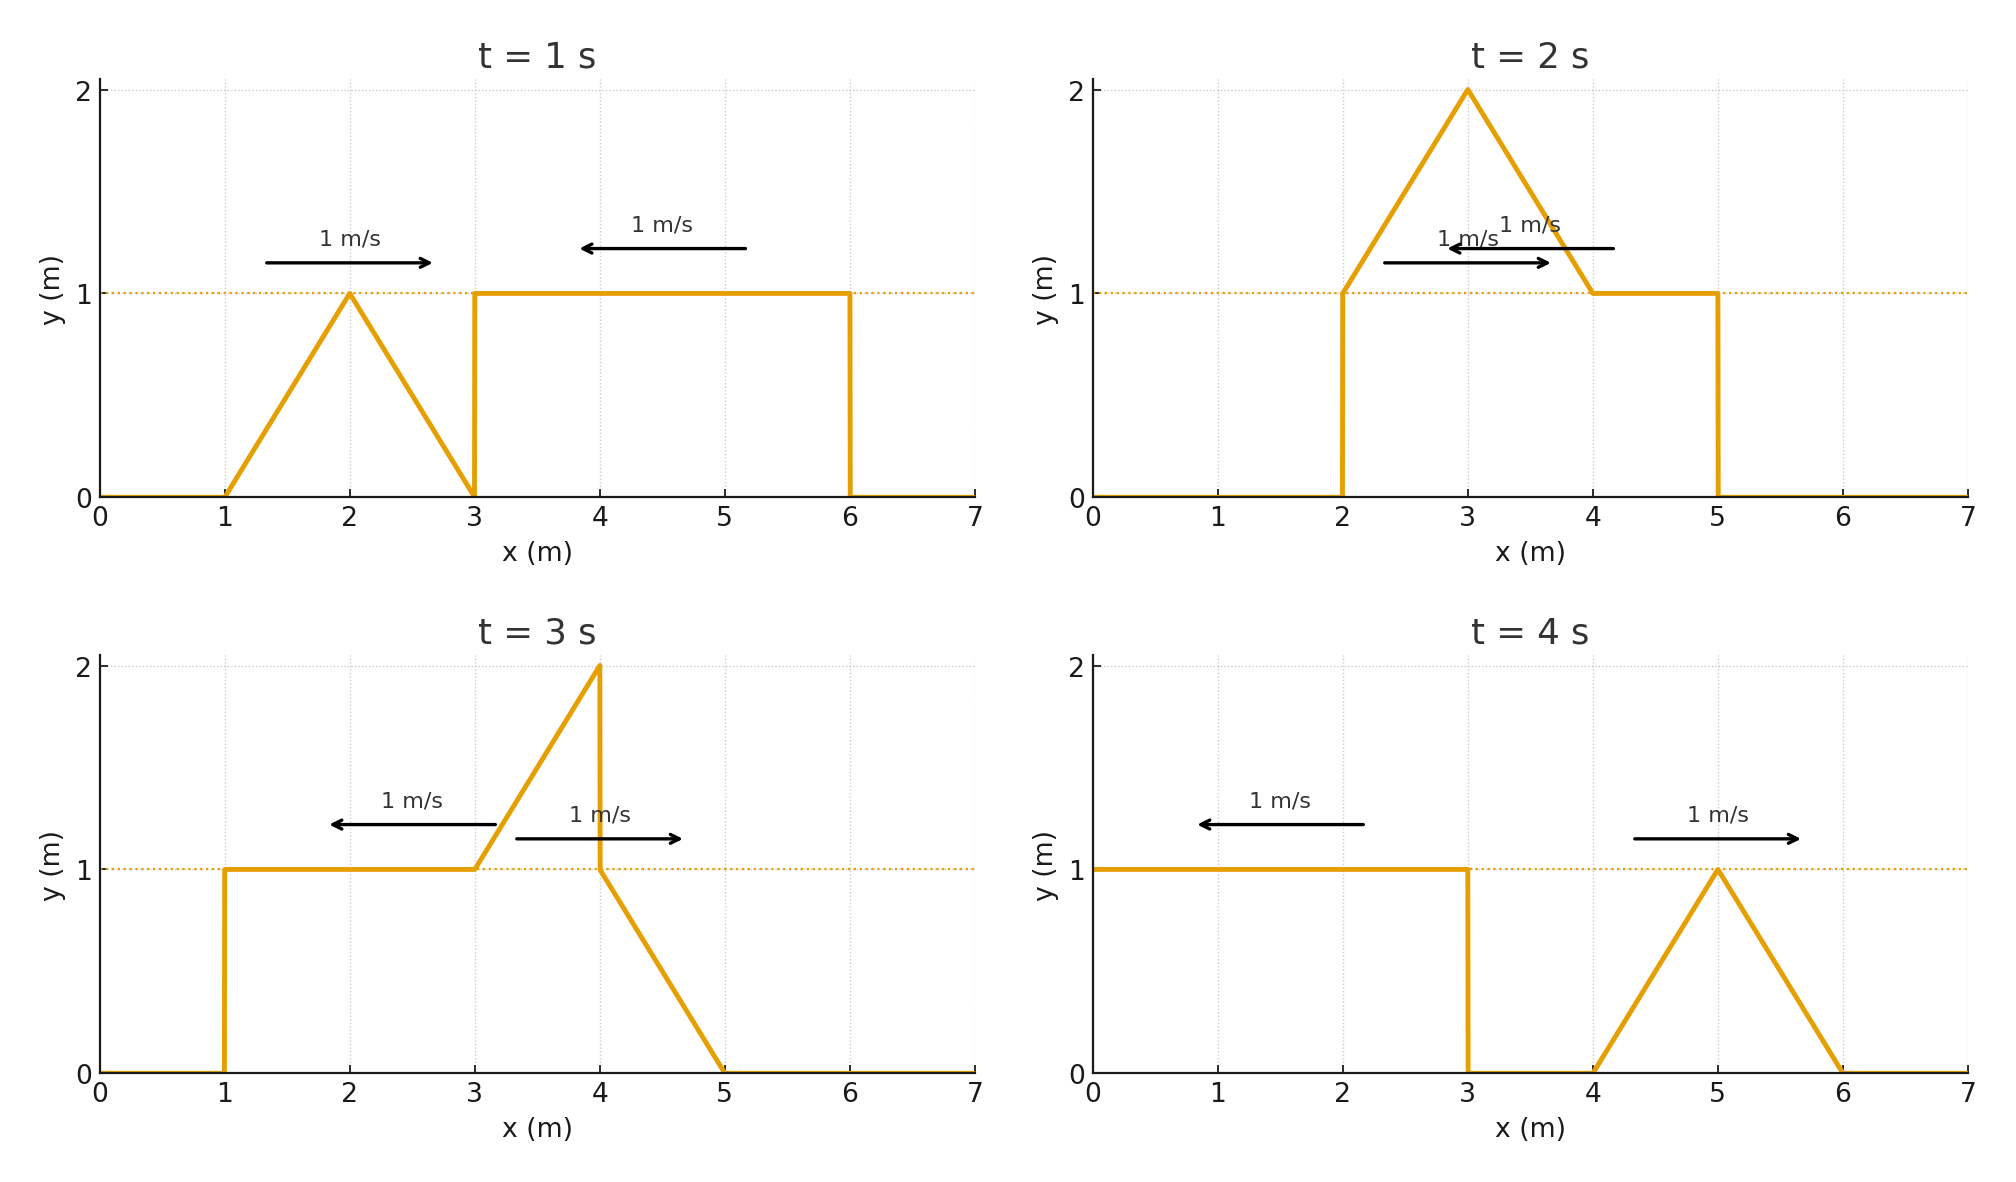
\includegraphics[width=0.6\textwidth]{Auxiliar_5_3}
        \captionof{figure}{Esquema del problema}
      \end{center}
    %%%%%%%%%%%%%%%%%%%%%%%%%%%%
    \begin{solution}
        \begin{enumerate}
            \item Se busca obtener una relación para los campos $E_{2}^{-}$ y  $E_{2}^{+}$ en función de de $d_{2}$, por tanto las expresiones de los campos eléctricos y magnéticos en general para los diferentes medios corresponden:
            \subsubsection*{\underline{Medio 1 : z $\leq$ d1}}
            \begin{align}
                E_{1}(z,t) &= (E_{1}^{+}e^{jwt}e^{-j\beta_{1} z} + E_{1}^{-}e^{jwt}e^{j\beta_{1} z})(\hat{x})
            \end{align}
            \begin{align}
                 H_{1}&= Y_{1}(\hat{z}) \times E_{1}(\hat{x})\\
                    H_{1} &= Y_{1}(E_{1}^{+}e^{jwt}e^{-j\beta_{1} z} - E_{1}^{-}e^{jwt}e^{j\beta_{1} z}) (\hat{y})
            \end{align}
            \subsubsection*{\underline{Medio 2: 
            $d_{1}$ $\leq$ z $\leq$ $d_{2}$}}
            \begin{align}
                E_{2}(z,t) &= (E_{2}^{+}e^{jwt}e^{-j\beta_{2} z} + E_{2}^{-}e^{jwt}e^{j\beta_{2} z})(\hat{x})
            \end{align}
            \begin{align}
                 H_{2}&= Y_{2}(\hat{z}) \times E_{2}(\hat{x})\\
                    H_{2} &= Y_{2}(E_{2}^{+}e^{jwt}e^{-j\beta_{2} z} - E_{1}^{-}e^{jwt}e^{j\beta_{2} z}) (\hat{y})
            \end{align}
            \subsubsection*{\underline{Medio 3: d2 $\leq$ z  $\leq$ 0 }}
            \begin{align}
                E_{3}(z,t) &= (E_{3}^{+}e^{jwt}e^{-j\beta_{3} z} + E_{3}^{-}e^{jwt}e^{j\beta_{3} z})(\hat{x})
            \end{align}
            \begin{align}
                 H_{3}&= Y_{3}(\hat{z}) \times E_{3}(\hat{x})\\
                    H_{3} &= Y_{3}(E_{3}^{+}e^{jwt}e^{-j\beta_{3} z} - E_{3}^{-}e^{jwt}e^{j\beta_{3} z}) (\hat{y})
            \end{align}
            Con lo que finalmente se obtienen las expresiones de campo eléctrico y intensidad magnetica para los 3 medios, el 4 es despreciable debido a la presencia de una pared con conductividad infinita (Reflexión total). Luego queremos relacionar $E_{2}^{+}$ y $E_{2}^{-}$ , es por esto que evaluaremos en la interfaz de los medios 2 y 3:
            \subsubsection*{\underline{Interfaz medio 2 y 3 (campo eléctrico)}}
            \begin{align}
                E_{2}(z=-d_{2}) = E_{3}(z=-d_{2})
            \end{align}
            Reemplazando y teniendo la consideración con los signos se tendrá que:
            \begin{align}
                (E_{2}^{+}e^{jwt}e^{j\beta_{2} d_{2}} + E_{2}^{-}e^{jwt}e^{-j\beta_{2} d_{2}})=(E_{3}^{+}e^{jwt}e^{j\beta_{3} d_{2}} + E_{3}^{-}e^{jwt}e^{-j\beta_{3} d_{2}}) 
            \end{align}
            A partir de ahora omitiremos en todas las expresiones los términos fasoriales asociados a el tiempo $e^{jwt}$ dado que no cambia con los cambios de medios por lo que no sera relevante.
            \begin{align}
                (E_{2}^{+}e^{j\beta_{2} d_{2}} + E_{2}^{-}e^{-j\beta_{2} d_{2}})=(E_{3}^{+}e^{j\beta_{3} d_{2}} + E_{3}^{-}e^{-j\beta_{3} d_{2}}) 
            \end{align}
            Necesitamos eliminar la dependencia de las amplitudes asociadas al medio 3. por lo que evaluando en z=0 , tenemos que:
            \begin{align}
                E_{3}(z=0,t) &= (E_{3}^{+}e^{-j\beta_{3} \cdot 0} + E_{3}^{-}e^{j\beta_{3} \cdot 0}) = 0\\
                      &= E_{3}^{+} + E_{3}^{-} = 0\\
                      &E_{3}^{+} = -E_{3}^{-}
            \end{align}
            Recordemos que lo igualamos a 0 , debido a la conductividad infinita de la interfaz y por tanto la no existencia de onda en el otro medio. Reemplazando esta condición sobre lo anterior:
            \begin{align}
                (E_{2}^{+}e^{j\beta_{2} d_{2}} + E_{2}^{-}e^{-j\beta_{2} d_{2}})&=(E_{3}^{+}e^{j\beta_{3} d_{2}} + E_{3}^{-}e^{-j\beta_{3} d_{2}})\\ 
                (E_{2}^{+}e^{j\beta_{2} d_{2}} + E_{2}^{-}e^{-j\beta_{2} d_{2}})&=E_{3}^{+}(e^{j\beta_{3}d_{2}}- e^{-j\beta_{3} d_{2}})\\
                (E_{2}^{+}e^{j\beta_{2} d_{2}} + E_{2}^{-}e^{-j\beta_{2} d_{2}})&=2 E_{3}^{+}jsen(\beta_{3}d_{s})
            \end{align}
            Con lo que reducimos a solo tener un $E_{3}^{+}$, con lo que debemos relacionar alguna otra expresión para reducirlo, usando la intensidad de campo magnético de la siguiente manera:
            \subsubsection*{\underline{Interfaz medio 2 y 3 (campo magnético)}}
            \begin{align}
                H_{2}(z=-d_{2}) &= H_{3}(z = - d_{2})\\
                Y_{2}(E_{2}^{+}e^{-j\beta_{2} z} - E_{1}^{-}e^{j\beta_{2} z}) &= Y_{3} (E_{3}^{+}e^{-j\beta_{3} z} - E_{3}^{-}e^{j\beta_{3} z})
            \end{align}
            Utilizamos la misma condición que obtuvimos de antes (\textit{Es decir que $E_{3}^{+} = -E_{3}^{-}$}):
            \begin{align}
                Y_{2}(E_{2}^{+}e^{-j\beta_{2} z} - E_{1}^{-}e^{j\beta_{2} z}) &=  Y_{3} E_{3}^{+}(e^{-j\beta_{3} z} + e^{j\beta_{3} z})\\
                 Y_{2}(E_{2}^{+}e^{-j\beta_{2} z} - E_{1}^{-}e^{j\beta_{2} z}) &=  Y_{3} 2E_{3}^{+}cos(\beta_{3}d_{2})   
            \end{align}
            Luego realizando la división se observa que queda expresada solo en términos de $E_{2}^{+} $ y $E_{2}^{-}$ con lo que podemos relacionarlos en función de parámetros conocidos, es decir:
            \begin{align}
                \frac{(E_{2}^{+}e^{j\beta_{2} d_{2}} + E_{2}^{-}e^{-j\beta_{2} d_{2}})}{Y_{2}(E_{2}^{+}e^{-j\beta_{2} z} - E_{1}^{-}e^{j\beta_{2} z})}= \frac{j tan(\beta_{3}d_{2})}{Y_{3}}
            \end{align}
            Luego despejando se logra obtener que 
            \begin{align}
                E_{2}^{-} = E_{2}^{+} \frac{e^{j\beta_{2}d_{2}} \left( \frac{Y_{2}}{Y_{3}} jtan(\beta_{3}d_{2}) -1\right)}{ e^{-j\beta_{2}d_{2}} \left( 1+ \frac{Y_{2}}{Y_{3}} j tan(\beta_{3}d_{2})\right)}
            \end{align}
            Con lo que finalmente se obtiene una expresión que relaciona los campos solo en función de la distancia $d_{2}$
            \item Se desea analizar la expresión anterior cuando $d_{2} = \frac{\lambda}{2}$ , por lo que evaluando de manera directa se tendrá:
            \begin{align}
                E_{2}^{-}=& E_{2}^{+} \frac{e^{j\beta_{2}\cdot \frac{\lambda}{2}} \left( \frac{Y_{2}}{Y_{3}} jtan(\beta_{3}\cdot \frac{\lambda}{2} )-1\right)}{ e^{-j\beta_{2}\cdot \frac{\lambda}{2}} \left( 1+ \frac{Y_{2}}{Y_{3}} j tan(\beta_{3}\cdot \frac{\lambda}{2})\right)}
            \end{align}
            Luego teniendo en consideración que :
            \begin{align}
                e^{\pm j\beta_{2}d_{2}} =  e^{\pm j \frac{2\pi}{\lambda} \cdot \frac{\lambda}{2}} = e^{\pm j \pi} = (-1)\\
                jtan(\beta_{3} d_{2}) = jtan(\pi) = 0
            \end{align}
            Relacionándolo con lo anterior sigue que:
            \begin{align}
                E_{2}^{-} &= E_{2}^{+} \frac{-1 \left( \frac{Y_{2}}{Y_{3}} \cdot 0 - 1\right)}{ -1 \left( 1+ \frac{Y_{2}}{Y_{3}} \cdot 0\right)}\\
                E_{2}^{-} &= - E_{2}^{+}
            \end{align}
            Con lo que tenemos un efecto similar al de una pared con conductividad infinita. Así calculamos el coeficiente de reflexión:
            \begin{align}
                \Gamma =& \frac{E_{2}^{-}}{E_{2}^{+}} e^{-2j\beta_{2}d_{2} }\\
                       =& (-1)
            \end{align}
            Donde si evaluamos obtenemos a priori lo que se esperaba el tener el efecto de una pared con conductividad infinita , esto principalmente porque tenemos amplitudes iguales solo con signos opuestos y por lo tanto tendremos además una reflexión con un desfase de $\pm$ $\pi$.
            \item Se busca relacionar las amplitudes para el medio 1 considerando la misma distancia para ($d_{2} = \lambda/4$) y relacionarlo con lo obtenido con anterioridad. Es \textbf{directo} ver que tenemos el mismo análisis anterior (\textit{Un error común es volver a calcularlo y perder mucho tiempo}) , por lo que directamente tenemos que:
            \begin{align}
                E_{1}^{-} = E_{1}^{+} \frac{e^{j\beta_{1}d_{1}} \left( \frac{Y_{1}}{Y_{2}} jtan(\beta_{2}d_{1}) -1\right)}{ e^{-j\beta_{1}d_{1}} \left( 1+ \frac{Y_{1}}{Y_{2}} j tan(\beta_{2}d_{1})\right)}
            \end{align}
            Con lo que tenemos para $d_{1} = d_{2} = \frac{\lambda}{2}$
            \begin{align}
                E_{1}^{-} = - E_{1}^{+} = - E_{0} 
            \end{align}
            Recordando que la amplitud de la onda incidente es conocida
            \item Luego buscamos obtener si las potencias de la onda incidente y reflejada son iguales \textbf{bajo las condiciones anteriores} , con lo tenemos lo siguiente:
            \begin{align}
                \langle S_{1}^{+} \rangle &= \frac{1}{2} Re( E_{1} \times H_{1}^{*})= \frac{1}{2}(E_{1}^{+})^{2}Y_{1} \hat{z} \\
                 \langle S_{1}^{-} \rangle &= \frac{1}{2} Re( E_{1} \times H_{1}^{*})= \frac{1}{2}(E_{1}^{-})^{2}Y_{1} \hat{z}  
            \end{align}
            En base a lo anterior se tendrá que $E_{1}^{+} = -E_{1}^{-} = - E_{0} $ , pero dado que tenemos la expresión cuadrado ,se observa finalmente que:
            \begin{align}
                \langle S_{1}^{+} \rangle = \langle S_{1}^{-} \rangle
            \end{align}
            Lo cual es consistente con la intuición.
        \end{enumerate}
    \end{solution}
     
    
%%%%%%%%%%%%%%%%%%%%%%%%%%%
\end{questions}
\newpage
%%%%%%%%%%%%%%%%%%%%%%%%%%%

\end{document}